\documentclass{if-beamer}

% --------------------------------------------------- %
%                  Presentation info	              %
% --------------------------------------------------- %
\title[Lecture 11]{Lecture 11}
\subtitle{Root Finding Methods: Open Methods}
\author{Instructor: Ashley Gannon}
\date{ISC3313 Fall 2021}
\logo{

\includegraphics[scale=0.08]{figures/FSULogo.png}
}
\subject{Presentation subject}

% --------------------------------------------------- %
%                    Title + Schedule                 %
% --------------------------------------------------- %
\begin{document}

\begin{frame}
  \titlepage
\end{frame}
% --------------------------------------------------- %
%                      Presentation                   %
% --------------------------------------------------- %
\section{Finishing up the Bisection method}
\begin{frame}
\frametitle{Pseudocode example}
\texttt{//Input: left bracket \textbf{a}, right bracket \textbf{b}}\\
\texttt{//Output: \textbf{void}, print the root to the screen} \\
\vspace{7pt}
\texttt{//check that there is a root in your initial domain}\\
\texttt{if f(a)f(b) >= 0} \\
\texttt{\qquad tell user to try a new domain and exit}\\
\vspace{7pt}
\texttt{//declare/define variables for the bisect method:}\\
\texttt{\qquad //tolerance, error, c\_old, and c\_new}\\
\vspace{7pt}
\texttt{loop while error>tolerance}\\
\texttt{find the mindpoint c\_new}\\
\texttt{//check if there is a root in the lower interval}\\
\texttt{\qquad if f(a)f(c) < 0}\\
\texttt{\qquad \qquad set b = c}\\
\texttt{\qquad else} \\
\texttt{\qquad \qquad set a = c} \\
\texttt{\qquad//Alternatively, you could check the upper interval first.}\\
\texttt{\qquad compute the error abs((c\_new-c\_old)/c\_new)} \\
\texttt{\qquad set c\_old = c\_new for the next iteration}\\
\texttt{print the root value to the screen}
\end{frame}

\begin{frame}
\frametitle{Let's code it!}

Take the next 15 minutes and try to write the Bisection method, \texttt{bisect.cpp}. If you finish writing it early, apply it to the function $f(m)$ from last lecture on the bounds $[140, 150]$. 
\\\vspace{7pt}
Post your code to the discussion board \textbf{Bisection method code}. Do NOT post screen shots of error messages or your code. Copy and paste the text from your code into the discussion board.

\end{frame}

\begin{frame}
Using our Bisection method code, we found that the root is 142.7 kg with an error of less than 0.00001\%. \\\vspace{7pt}

How confident would you be using that \textbf{initial graphical approximation} from the last lecture: the maximum cutoff weight for this bungee jump is 145 kg/ 320lbs?
\end{frame}

\begin{frame}
Using our Bisection method code, we found that the root is 142.7 kg with an error of less than 0.00001\%. \\\vspace{7pt}

How confident would you be using that \textbf{initial graphical approximation} from the last lecture: Telling your boss the maximum cutoff weight for this bungee jump is 145 kg/ 320lbs?\\\vspace{7pt}

How confident would you be using the result from the bisection method?
\end{frame}



\section{Concept review}

\begin{frame}
\frametitle{Bracketing methods}
\begin{minipage}{0.5\textwidth}
	For the \textit{bracketing methods} we discussed last class, we saw that \\\vspace{7pt}
	\begin{itemize}
		\item the root is located within an interval prescribed by a lower and an upper bound.\\\vspace{7pt}
		\item  Repeated application of these methods always results in closer estimates of the true value of the root.\\\vspace{7pt}
		\item Such methods are said to be convergent because they move closer to the true solution as the computation progresses.
	\end{itemize} 
\end{minipage}
\begin{minipage}{0.5\textwidth}
	\begin{figure}
		\centering
		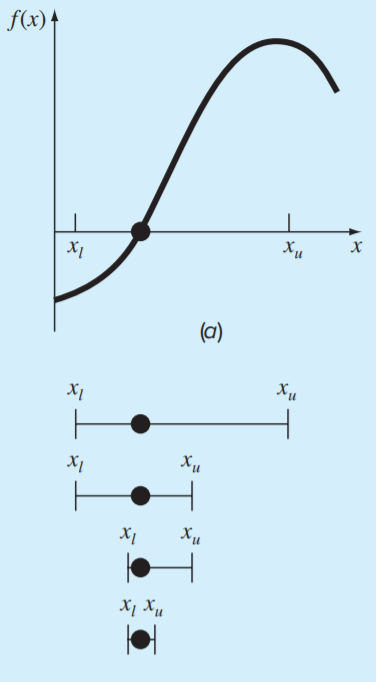
\includegraphics[width=.55\textwidth]{figures/bisection}
	\end{figure}
\end{minipage}
\end{frame}	

\begin{frame}
\frametitle{Open methods}
\begin{minipage}{0.5\textwidth}
	The \textit{open methods} described in this lecture and the next lecture\\\vspace{7pt} 
	\begin{itemize}
		\item will sometimes only require a single starting value \\\vspace{2pt}
		\item will sometimes require two starting values, but they do not necessarily bracket the root \\\vspace{2pt}
		\item will sometimes diverge away from the true solution as the computation progresses \\\vspace{2pt}
	\end{itemize}
\end{minipage} 
\begin{minipage}{0.5\textwidth}
	\centering
	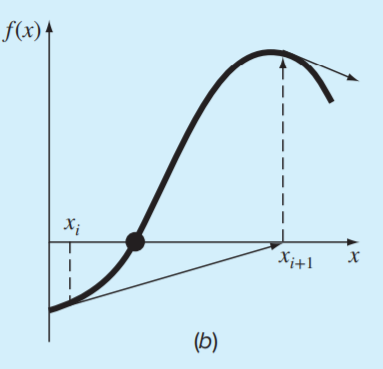
\includegraphics[width = 0.9\textwidth]{figures/diverging}
\end{minipage}
\end{frame}


\begin{frame}
\frametitle{Open methods}
\begin{minipage}{0.5\textwidth}
	The \textit{open methods} described in this lecture and the next lecture\\\vspace{7pt} 
	\begin{itemize}
		\item will sometimes only require a single starting value \\\vspace{2pt}
		\item will sometimes require two starting values, but they do not necessarily bracket the root \\\vspace{2pt}
		\item will sometimes diverge away from the true solution as the computation progresses \\\vspace{2pt}
		\item will converge quicker than the bracketing methods when they converge.
	\end{itemize}
\end{minipage} 
\begin{minipage}{0.5\textwidth}
	\centering
	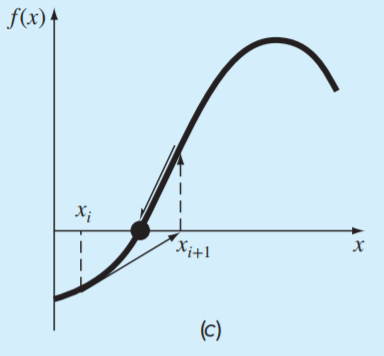
\includegraphics[width = 0.9\textwidth]{figures/converging}
\end{minipage}
\end{frame}

	
\section{Simple Fixed-Point Iteration}
\begin{frame}[t]
\frametitle{Simple fixed-point iteration method}
Open methods employ a formula to predict the root. Such a formula can
be developed for \textit{simple fixed-point iteration} (also known as \textit{one-point iteration} or \textit{successive substitution}) by rearranging the function $f(x) = 0$ so that $x$ is on the left-hand
side of the equation. \\\vspace{7pt}

\end{frame}

\begin{frame}[t]
\frametitle{Simple fixed-point iteration method}
Open methods employ a formula to predict the root. Such a formula can
be developed for \textit{simple fixed-point iteration} (also known as \textit{one-point iteration} or \textit{successive substitution}) by rearranging the function $f(x) = 0$ so that $x$ is on the left-hand
side of the equation. \\\vspace{7pt}

This transformation can be accomplished either by algebraic manipulation or by simply adding $x$ to both sides of the original equation. The utility of this is that it provides a formula to predict a new value of $x$ as a function of an old value of $x$.  \\\vspace{7pt}

\end{frame}

\begin{frame}
\frametitle{Simple fixed-point iteration method}
Open methods employ a formula to predict the root. Such a formula can
be developed for \textit{simple fixed-point iteration} (also known as \textit{one-point iteration} or \textit{successive substitution}) by rearranging the function $f(x) = 0$ so that $x$ is on the left-hand
side of the equation. \\\vspace{7pt}

This transformation can be accomplished either by algebraic manipulation or by simply adding $x$ to both sides of the original equation. The utility of this is that it provides a formula to predict a new value of $x$ as a function of an old value of $x$.  \\\vspace{7pt}

Therefore, given an initial guess at the root $x_i$, the function can be used to compute a new estimate $x_{i+1}$. \\\vspace{7pt} 
Let's consider the function
$$f(x) = e^{-x} -x$$ 
If we let $f(x) = 0$ and move $x$ to our left-hand side, we end up with
$$x = e^{-x}$$
The $x$ on our left-hand side becomes $x_{i+1}$, the $x$ on our right-hand side becomes $x_{i}$. This formula now predicts a new value of $x$ as a function of the old value of $x$.
$$x_{i+1} = e^{-x_i}$$ 
\end{frame}

\begin{frame}
\frametitle{Simple fixed-point iteration method}
Thinking about this graphically, \\\vspace{5pt}
\begin{minipage}{0.5\textwidth}
	\begin{figure}
		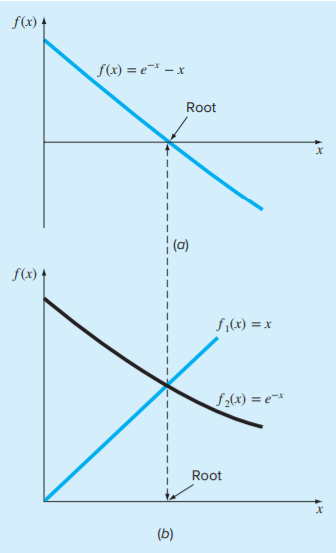
\includegraphics[width = 0.75\textwidth]{figures/graphic}
	\end{figure}
\end{minipage}
\begin{minipage}{0.5\textwidth}
	The x values corresponding to the intersections of these functions represent the roots of $f(x)=0$. Splitting the function into two component parts and plotting them is called the \textit{two curve method}.
\end{minipage}
 
\end{frame}

\begin{frame}[t]
\frametitle{Simple fixed-point iteration method}
Use simple fixed-point iteration to locate the root of $f(x) = e^{-x}-x$.
$$x_{i+1} = e^{-x_i}$$
\begin{table}
	\begin{tabular}{c | c | c}
		i & $x_i$ & $x_{i+1}$ \\
		\hline
		0 & 0.000 & $x_2 = e^{-x_0} = 1.000$\\ 
	\end{tabular}
\end{table}
\end{frame}

\begin{frame}[t]
\frametitle{Simple fixed-point iteration method}
Use simple fixed-point iteration to locate the root of $f(x) = e^{-x}-x$.
$$x_{i+1} = e^{-x_i}$$
\begin{table}
	\begin{tabular}{c | c | c}
		i & $x_i$ & $x_{i+1}$ \\
		\hline
		0 & 0.000 & $x_1 = e^{-x_0} = 1.000$\\ 
		1 & 1.000 & $x_2 = e^{-1.000}=0.3679$ \\ 
	\end{tabular}
\end{table}
\end{frame}

\begin{frame}[t]
\frametitle{Simple fixed-point iteration method}
Use simple fixed-point iteration to locate the root of $f(x) = e^{-x}-x$.
$$x_{i+1} = e^{-x_i}$$
\begin{table}
	\begin{tabular}{c | c | c}
		i & $x_i$ & $x_{i+1}$ \\
		\hline
		0 & 0.000 & $x_1 = e^{-x_0} = 1.000$\\ 
		1 & 1.000 & $x_2 = e^{-1.000}= 0.3679$ \\
		2 & 0.3679 & $x_3 = e^{-0.3679} =  0.6922$ \\ 
	\end{tabular}
\end{table}
\end{frame}

\begin{frame}[t]
\frametitle{Simple fixed-point iteration method}
Use simple fixed-point iteration to locate the root of $f(x) = e^{-x}-x$.
$$x_{i+1} = e^{-x_i}$$
\begin{table}
	\begin{tabular}{c | c | c}
		i & $x_i$ & $x_{i+1}$ \\
		\hline
		0 & 0.000 & $x_1 = e^{-x_0} = 1.000$\\ 
		1 & 1.000 & $x_2 = e^{-1.000}= 0.3679$ \\
		2 & 0.3679 & $x_3 = e^{-0.3679} =  0.6922$ \\ 
		3 & 0.6922 & $x_4 = e^{-0.6922} = 0.5005$ \\	
	\end{tabular}
\end{table}
\end{frame}

\begin{frame}[t]
\frametitle{Simple fixed-point iteration method}
Use simple fixed-point iteration to locate the root of $f(x) = e^{-x}-x$.
$$x_{i+1} = e^{-x_i}$$
\begin{table}
\begin{tabular}{c | c | c}
i & $x_i$ & $x_{i+1}$ \\
\hline
0 & 0.000 & $x_1 = e^{-x_0} = 1.000$\\ 
1 & 1.000 & $x_2 = e^{-1.000}= 0.3679$ \\
2 & 0.3679 & $x_3 = e^{-0.3679} =  0.6922$ \\ 
3 & 0.6922 & $x_4 = e^{-0.6922} = 0.5005$ \\
4 & 0.5005 & $x_5 = e^{-0.5005} =  0.6062$\\	
\end{tabular}
\end{table}
\end{frame}

\begin{frame}[t]
\frametitle{Simple fixed-point iteration method}
Use simple fixed-point iteration to locate the root of $f(x) = e^{-x}-x$.
$$x_{i+1} = e^{-x_i}$$
\begin{table}
	\begin{tabular}{c | c | c}
		i & $x_i$ & $x_{i+1}$ \\
		\hline
		0 & 0.000 & $x_1= e^{-x_0} = 1.000$\\ 
		1 & 1.000 & $x_2 = e^{-1.000}= 0.3679$ \\
		2 & 0.3679 & $x_3 = e^{-0.3679} =  0.6922$ \\ 
		3 & 0.6922 & $x_4 = e^{-0.6922} = 0.5005$ \\
		4 & 0.5005 & $x_5 = e^{-0.5005} =  0.6062$\\	
		5 & 0.6062 & $x_6 = e^{-0.6062} = 0.5454$\\
		6 & 0.5454 & $x_7 = e^{-0.5454} = 0.5796$ \\
		7 & 0.5796 & $x_8 = e^{-0.5796} = 0.5601$ \\
		8 & 0.5601 & $x_9 = e^{-0.5601} = 0.5711$ \\
		9 & 0.5711 & $x_{10} =e^{-0.5711} = 0.5649$ 
	\end{tabular}
\end{table}

Notice each iteration brings the estimate closer to the true value of the root: 0.56714329.
\end{frame}

\begin{frame}[t]
\frametitle{Simple fixed-point iteration method}
Use simple fixed-point iteration to locate the root of $f(x) = e^{-x}-x$.
$$x_{i+1} = e^{-x_i}$$
\begin{minipage}{0.7\textwidth}
	\begin{table}
		\begin{tabular}{c | c | c | c}
			i & $x_i$ & $x_{i+1}$ & $\frac{\epsilon_i}{\epsilon_{i-1}}$\\
			\hline
			0 & 0.000 & $x_1= e^{-x_0} = 1.000$ &  --\\ 
			1 & 1.000 & $x_2 = e^{-1.000}= 0.3679$ & 0.763 \\
			2 & 0.3679 & $x_3 = e^{-0.3679} =  0.6922$ & 0.460 \\ 
			3 & 0.6922 & $x_4 = e^{-0.6922} = 0.5005$ & 0.628 \\
			4 & 0.5005 & $x_5 = e^{-0.5005} =  0.6062$ & 0.533\\	
			5 & 0.6062 & $x_6 = e^{-0.6062} = 0.5454$ & 0.586\\
			6 & 0.5454 & $x_7 = e^{-0.5454} = 0.5796$ & 0.556\\
			7 & 0.5796 & $x_8 = e^{-0.5796} = 0.5601$ & 0.573 \\
			8 & 0.5601 & $x_9 = e^{-0.5601} = 0.5711$ & 0.564\\
			9 & 0.5711 & $x_{10} =e^{-0.5711} = 0.5649$ & 0.569
		\end{tabular}
	\end{table}
\end{minipage}
\begin{minipage}{0.3\textwidth}
	Notice that the true percent relative error  $\frac{\epsilon_i}{\epsilon_{i-1}}$ for each iteration is roughly proportional to the error from the previous iterations.\\\vspace{3pt}
	
	This property is called \textit{linear convergence}, and it is characteristic of fixed-point
	iteration.
\end{minipage}

\end{frame}

\section{Deriving the Newton-Raphson method}
\begin{frame}
\frametitle{Deriving the Newton-Raphson method}
The Newton-Raphson method is one of the most widely used of all root-locating methods. \\
\begin{minipage}{0.5\textwidth}
	\begin{itemize}
		\item  If the initial guess at the root is $x_i$, a tangent can be extended from the point $(x_i,f(x_i))$
		\item  The point where this tangent crosses the x axis usually represents an improved estimate of the root.
		\item  The point where this tangent ($f'(x)$) crosses the x axis usually represents an improved estimate of the root.
	\end{itemize}
\end{minipage}
\begin{minipage}{0.5\textwidth}
	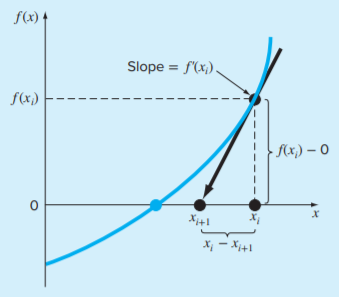
\includegraphics[width = 0.8\textwidth]{figures/NR}
\end{minipage}
\\\vspace{5pt}
Algebraically, the first derivative at $x$ is equivalent to the slope
$$f'(x_i) = \frac{f(x_i)-0}{x_i-x_{i+1}}$$
Which can be re-arranged to the form
$$x_{i+1} = x_i - \frac{f(x_i)}{f'(x_i)}$$
which is called the \textit{Newton-Raphson formula}.
\end{frame}

\section{Newton Raphson method}
\begin{frame}
\frametitle{Example problem}
Let's look at this example again...\\\vspace{3pt}
Use the Newton-Raphson method to locate the root of $f(x) = e^{-x}-x$.The derivative of $f(x)$ is $f'(x) = -e^{-x}-1$.
$$x_{i+1} = x_i - \frac{f(x_i)}{f'(x_i)} =  x_i - \frac{e^{-x_i}-x_i}{-e^{-x_i}-1}$$
\begin{table}
	\begin{tabular}{c | c | c}
		i & $x_i$ & $x_{i+1}$ \\
		\hline
		0 & 0.000000000 & $x_1= x_0 - \frac{f(x_0)}{f'(x_0)} = 0.500000000$\\ 
	\end{tabular}
\end{table}

\end{frame}

\begin{frame}
\frametitle{Example problem}
Let's look at this example again...\\\vspace{3pt}
Use the Newton-Raphson method to locate the root of $f(x) = e^{-x}-x$.The derivative of $f(x)$ is $f'(x) = -e^{-x}-1$.
$$x_{i+1} = x_i - \frac{f(x_i)}{f'(x_i)} =  x_i - \frac{e^{-x_i}-x_i}{-e^{-x_i}-1}$$
\begin{table}
	\begin{tabular}{c | c | c}
		i & $x_i$ & $x_{i+1}$ \\
		\hline
		0 & 0.000000000 & $x_1= x_0 - \frac{f(x_0)}{f'(x_0)} = 0.500000000$\\ 
		1 & 0.500000000 & $x_2= x_1 - \frac{f(x_1)}{f'(x_1)} = 0.566311003$ \\
	\end{tabular}
\end{table}

\end{frame}

\begin{frame}
\frametitle{Example problem}
Let's look at this example again...\\\vspace{3pt}
Use the Newton-Raphson method to locate the root of $f(x) = e^{-x}-x$.The derivative of $f(x)$ is $f'(x) = -e^{-x}-1$.
$$x_{i+1} = x_i - \frac{f(x_i)}{f'(x_i)} =  x_i - \frac{e^{-x_i}-x_i}{-e^{-x_i}-1}$$
\begin{table}
	\begin{tabular}{c | c | c}
		i & $x_i$ & $x_{i+1}$ \\
		\hline
		0 & 0.000000000 & $x_1= x_0 - \frac{f(x_0)}{f'(x_0)} = 0.500000000$\\ 
		1 & 0.500000000 & $x_2= x_1 - \frac{f(x_1)}{f'(x_1)} = 0.566311003$ \\
		2 & 0.566311003	 & $x_3= x_2 - \frac{f(x_2)}{f'(x_2)} = 0.567143165	$ 
	\end{tabular}
\end{table}

\end{frame}

\begin{frame}
\frametitle{Example problem}
Let's look at this example again...\\\vspace{3pt}
Use the Newton-Raphson method to locate the root of $f(x) = e^{-x}-x$.The derivative of $f(x)$ is $f'(x) = -e^{-x}-1$.
$$x_{i+1} = x_i - \frac{f(x_i)}{f'(x_i)} =  x_i - \frac{e^{-x_i}-x_i}{-e^{-x_i}-1}$$
\begin{table}
	\begin{tabular}{c | c | c}
		i & $x_i$ & $x_{i+1}$ \\
		\hline
		0 & 0.000000000 & $x_1= x_0 - \frac{f(x_0)}{f'(x_0)} = 0.500000000$\\ 
		1 & 0.500000000 & $x_2= x_1 - \frac{f(x_1)}{f'(x_1)} = 0.566311003$ \\
		2 & 0.566311003	 & $x_3= x_2 - \frac{f(x_2)}{f'(x_2)} = 0.567143165	$ \\ 
		3 & 0.567143165	 & $x_4= x_3 - \frac{f(x_3)}{f'(x_3)} = 0.567143290$	 \\
	\end{tabular}
\end{table}

\end{frame}


\begin{frame}
\frametitle{Example problem}
Let's look at this example again...\\\vspace{3pt}
Use the Newton-Raphson method to locate the root of $f(x) = e^{-x}-x$.The derivative of $f(x)$ is $f'(x) = -e^{-x}-1$.
$$x_{i+1} = x_i - \frac{f(x_i)}{f'(x_i)} =  x_i - \frac{e^{-x_i}-x_i}{-e^{-x_i}-1}$$
\begin{table}
	\begin{tabular}{c | c | c}
		i & $x_i$ & $x_{i+1}$ \\
		\hline
		0 & 0.000000000 & $x_1= x_0 - \frac{f(x_0)}{f'(x_0)} = 0.500000000$\\ 
		1 & 0.500000000 & $x_2= x_1 - \frac{f(x_1)}{f'(x_1)} = 0.566311003$ \\
		2 & 0.566311003	 & $x_3= x_2 - \frac{f(x_2)}{f'(x_2)} = 0.567143165	$ \\ 
		3 & 0.567143165	 & $x_4= x_3 - \frac{f(x_3)}{f'(x_3)} = 0.567143290$	 \\
		4 & 0.567143290 &
	\end{tabular}
\end{table}
Notice each iteration brings the estimate closer to the true value of the root: 0.56714329, and at a much faster rate than the simple-fixed point method.
\end{frame}

\begin{frame}
\frametitle{Stopping criteria}
We need to think about the stopping criteria for the Newton-Raphson method. Common stopping criteria used are 
\begin{itemize}
	\item checking if the function value is close to $0$, $|f(x_i)|< \epsilon$,
	\item checking if the difference between successive iterations is small, $|x_{i+1}-x_i| <\epsilon$,
	\item Capping the number of iterations, $i > maxIter$. 
\end{itemize}
The second option is often used instead of or in conjunction with the first option because it is possible for $f(x_i)$ to be close to $0$, but $x_i$ is not close to the root $x^*$. Additionally, Newton's method is not guaranteed to converge. Therefore, you should always include an iteration cap.
\end{frame}

\begin{frame}
\frametitle{Sign-off activity}
Write a pseudocode for the Newton-Raphson method based on the example and the stopping criteria outlined in the previous slides.
\\\vspace{10pt} 
When you are finished, post your draft in the discussion board \textbf{Newton-Raphson Pseudocode}. 
\end{frame}

\end{document}
